
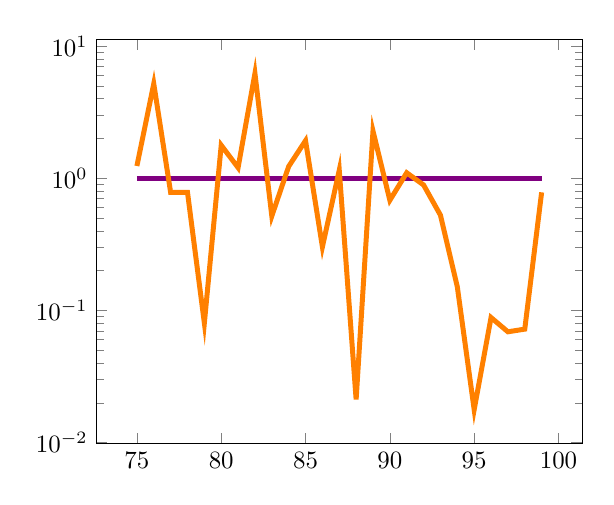
\begin{tikzpicture}[scale=0.9]
\begin{semilogyaxis}
\addplot[color=violet,line width=2pt] coordinates {(75,1.0)(76,1.0)(77,1.0)(78,1.0)(79,1.0)(80,1.0)(81,1.0)(82,1.0)(83,1.0)(84,1.0)(85,1.0)(86,1.0)(87,1.0)(88,1.0)(89,1.0)(90,1.0)(91,1.0)(92,1.0)(93,1.0)(94,1.0)(95,1.0)(96,1.0)(97,1.0)(98,1.0)(99,1.0)};
\addplot[color=orange,line width=2pt] coordinates {(75,1.2380162506559278)(76,5.188404299202283)(77,0.782567667616828)(78,0.7830360342709969)(79,0.08018426072068464)(80,1.7775828909033573)(81,1.2022932505283686)(82,6.2165805780626595)(83,0.517523619010797)(84,1.2285226215628358)(85,1.9255889004679672)(86,0.30249979948308037)(87,1.1510422729709011)(88,0.021178669591749102)(89,2.2789702680684734)(90,0.6815532630837864)(91,1.100666623122917)(92,0.889682124955427)(93,0.5257227003565701)(94,0.15081514459257384)(95,0.017746708725184978)(96,0.08830577066445135)(97,0.06889969612550335)(98,0.07215904757230174)(99,0.782639756105992)};

\end{semilogyaxis}
\end{tikzpicture}
